\documentclass[]{article}
\usepackage[a4paper, total={15cm,23cm}]{geometry}
\usepackage{fancyhdr}
\usepackage{graphicx}
\usepackage{amsmath}
\usepackage{amssymb}
%\usepackage[dvipsnames]{xcolor}
\usepackage{tikz}
\usepackage{verbatim}
\usepackage{tcolorbox}
\usepackage{textcomp}
\usepackage{xcomment}
\usepackage{xstring}
%opening
\title{RC Concepts in Current}
\author{Benjamin Bauml}
\date{Winter 2024}
\pagestyle{fancy}
\rhead{PH 223}
\chead{Winter 2024}
\lhead{Week 10}

% Version 2024-02-21
% Changes
% 2024-02-21 Added xstring package to enable smooth implementation of new \ModePage command.
% For Assignment, leave Purpose as 1. For Worksheet, set to 2. For Student Solution, set to 3. For Teacher Solution, set to 4.
\newcommand{\Purpose}{4}

\newcommand{\Exclusion}{0}
\newcommand{\PageTurn}{0}
\newcommand{\GrayProb}{0}
\newcommand{\Tipsy}{0}

% Assignment
\if\Purpose1
\renewcommand{\Exclusion}{1}
\fi
% Worksheet
\if\Purpose2
\renewcommand{\Exclusion}{1}
\renewcommand{\PageTurn}{1}
\fi
% Student Solution
\if\Purpose3
\renewcommand{\PageTurn}{1}
\renewcommand{\GrayProb}{1}
\fi
% Teaching Copy
\if\Purpose4
\renewcommand{\PageTurn}{1}
\renewcommand{\GrayProb}{1}
\renewcommand{\Tipsy}{1}
\fi

\if\Exclusion1
\xcomment{Title,Problem,ProblemSub,PassFig}
\fi

\def \NewQ {0}
\def \PForce {0}
\newcommand{\MaybePage}[1]{
	\def \PForce {#1}
	\if\PForce1
		\newpage
	\else
		\if\NewQ0
		\gdef \NewQ {\PageTurn}
		\else
		\newpage
		\fi
	\fi
}

\newcommand{\ModePage}[1]{
	\IfSubStr{#1}{\Purpose}{\newpage}{}
}

\newenvironment{Problem}[2][0]{%The first argument is optional, and if it is set to 1, the \newpage will be forced.
\MaybePage{#1}
\section*{#2}
\if\GrayProb1
\begin{tcolorbox}[colback=lightgray,colframe=lightgray,sharp corners,boxsep=1pt,left=0pt,right=0pt,top=0pt,bottom=0pt,after skip=2pt]
\else
\begin{tcolorbox}[colback=white,colframe=white,sharp corners,boxsep=1pt,left=0pt,right=0pt,top=0pt,bottom=0pt,after skip=2pt]
\fi
}{
\end{tcolorbox}\noindent
}

\newenvironment{ProblemSub}[1][0]{%The argument is optional, and if a string of numbers is entered into it, it will force a \newpage in any \Purpose that shows up in the string. For example, "13" would lead to the newpage being forced in modes 1 and 3.
\ModePage{#1}
\if\GrayProb1
\begin{tcolorbox}[colback=lightgray,colframe=lightgray,sharp corners,boxsep=1pt,left=0pt,right=0pt,top=0pt,bottom=0pt,after skip=2pt]
\else
\begin{tcolorbox}[colback=white,colframe=white,sharp corners,boxsep=1pt,left=0pt,right=0pt,top=0pt,bottom=0pt,after skip=2pt]
\fi
}{
\end{tcolorbox}\noindent
}

\newenvironment{PassFig}{\begin{figure}[h]}{\end{figure}}

\newcommand{\TeachingTips}[1]{
\if\Tipsy1
\begin{tcolorbox}[colback=lightgray,colframe=black]
#1
\end{tcolorbox}
\fi
}

\newenvironment{Title}{\maketitle}{}

\begin{document}
\begin{Title}
\begin{center}
	This problem is borrowed from Chapter 29 of the \textit{Student Workbook} for \textit{Physics for Scientists and Engineers}.
\end{center}
\end{Title}

\begin{Problem}{Activity}
	The capacitor in this circuit was initially charged, then the switch was closed. At this instant of time, the potential difference across the resistor is $ \Delta V_{R} = 4 $ V.
\end{Problem}
\begin{PassFig}
	\centering
	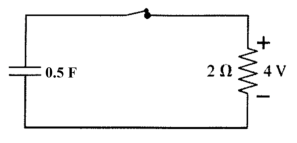
\includegraphics[scale=1.2]{RC_Concepts_Circuit}
\end{PassFig}
\begin{ProblemSub}
	(a) At this instant of time, what is the current through the resistor? %What is the current through the space between the capacitor plates?
\end{ProblemSub}
The current through the resistor at the instant the switch closes is
\[
	I_{0} = \frac{\Delta V_{R}}{R} = \frac{4\text{ V}}{2\text{ \textohm}} = 2\text{ A}.
\]
%No charge actually crosses the gap between the plates, so $ I_{through} = 0 $ A.
\begin{ProblemSub}
	(b) What is the current through the resistor over time?
\end{ProblemSub}
A discharging RC circuit has current of the form
\[
	I(t) = I_{0} e^{-t/\tau}.
\]
We just found $ I_{0} $, and for the given circuit, $ \tau = RC = (2\text{ \textohm})(\frac{1}{2}\text{ F}) = 1 $ s. As such,
\[
	I(t) = (2\text{ A}) e^{-t/(1\text{ s})}.
\]
\begin{ProblemSub}
	(c) What is the charge in the capacitor over time?
\end{ProblemSub}
A discharging RC circuit has charge of the form
\[
	Q(t) = Q_{0}e^{-t/\tau}.
\]
The initial charge $ Q_{0} = \Delta V_{C} C $, and the initial voltage difference across the capacitor must be $ \Delta V_{C} = 4 $ V by Kirchhoff's loop law. As such, $ Q_{0} = (4\text{ V})(\frac{1}{2}\text{ F}) = 2\text{ C} $, and the charge varies over time as
\[
	Q(t) = (2\text{ C})e^{-t/(1\text{ s})}.
\]
\begin{ProblemSub}
(d) If the capacitor consists of two parallel plates of area $ A $, symbolically calculate the electric flux between them, and the time derivative of this flux. %Use this to obtain the displacement current.
\end{ProblemSub}
Assuming uniform distribution of charge over the plate, the surface charge density across the positive side is
\[
	\sigma(t) = \frac{Q(t)}{A} = \frac{Q_{0}}{A}e^{-t/\tau}.
\]
Thus, the electric field magnitude between the plates is
\[
	E = \frac{\sigma(t)}{\epsilon_{0}} = \frac{Q_{0}}{A\epsilon_{0}}e^{-t/\tau}.
\]
As such, the flux through the cross-sectional area $ A $ of the region between the plates is
\[
	\Phi_{e} = EA = \frac{Q_{0}}{\epsilon_{0}}e^{-t/\tau}.
\]
	This flux changes in time as
\[
	\frac{d\Phi_{e}}{dt} = -\frac{Q_{0}}{\tau\epsilon_{0}}e^{-t/\tau} = -\frac{Q_{0}}{RC\epsilon_{0}}e^{-t/\tau} = -\frac{\Delta V_{R}}{R\epsilon_{0}}e^{-t/\tau} = -\frac{I_{0}}{\epsilon_{0}}e^{-t/\tau}.
\]
\begin{comment}
Displacement current is defined to be $ I_{disp} = \epsilon_{0}\frac{d\Phi_{e}}{dt} $, so
\[
	I_{disp}(t) = -I_{0}e^{-t/\tau} = -I(t).
\]
We see that the magnitude of displacement current is the same as the magnitude of true current in the system over time. The negative sign indicates that the displacement current is opposite the electric field in the capacitor (caused by the field decreasing). This would make the current flow toward the positive plate, and actual current is leaving this plate down the wire as the capacitor discharges, so the direction of the displacement current is actually consistent with the direction of true current in the system.
\end{comment}
\end{document}
